%% Internal working report: the signal-loss audit, described in full.
%% Same section structure as paper/pilot.tex. Not for submission.
\documentclass[preprint,12pt,authoryear]{elsarticle}

\usepackage[T1]{fontenc}
\usepackage[utf8]{inputenc}
\usepackage{lmodern}
\usepackage{amsmath,amssymb}
\usepackage{booktabs}
\usepackage{array}
\usepackage{graphicx}
\usepackage{xcolor}
\usepackage{microtype}
\usepackage{tikz}
\usetikzlibrary{positioning,arrows.meta}
\usepackage[hidelinks]{hyperref}

\graphicspath{{../../paper/figures/}}
\setlength{\emergencystretch}{2em}

\journal{working report, not for submission}

\begin{document}

\begin{frontmatter}

  \title{Noise Removal versus Signal Loss in Network Filtering of Daily GNSS Time Series: Internal Working Report}

  \author{H. O\u{g}uz Bolat}
  \ead{oguz.bolat@std.yildiz.edu.tr}
  \affiliation{organization={Department of Geomatics Engineering, Y{\i}ld{\i}z Technical University},
    city={Istanbul},
  country={T\"urkiye}}

  \begin{abstract}
    This report describes, in full, a signal-loss audit of network filters for daily GNSS position time series, and reports its results without drawing conclusions from them. Daily IGS20 solutions of the Nevada Geodetic Laboratory for 1,251 stations in and around California are reduced to residuals by removing a trajectory model fitted on 2008--2019. Seventeen filter configurations from three families are audited: target-inclusive filters, which use the target station in its own estimate (network stack, sub-regional probabilistic PCA, robust weighted median); distance-excluded filters, which use every station beyond a radius $R$; and leave-one-out filters over nearest neighbours, from weighted means and ridge regression to a learned kernel and a space--time attention network, the last also trained with planted transients. Each filter is scored on two noise measures, the reduction in short-period scatter and the leave-one-out reconstruction error, and on two signal measures, the fraction of a planted transient that it keeps and the spurious signal it creates outside the transient. Transients are planted as idealised Gaussian fields of 10--100~km width and as fault-slip events on the SCEC Community Fault Model; real earthquake offsets and the Ridgecrest postseismic displacement are scored as well. On the test years (2022 to September 2026), the mean of every station beyond $R$ (far stack) removes 22.7\% of the short-period scatter at $R = 0$ and keeps 0.98 and 0.83 of 25- and 100-km transients; the weighted mean of the 16 nearest stations removes 14.1\% and keeps 0.25 and 0.00. The reconstruction errors of the attention network, its transient-trained version and the learned kernel over 256 neighbours are not distinguishable from that of the far stack, and each keeps less planted signal. Results on the validation years (2020--2021) are given alongside where they differ.
  \end{abstract}

  \begin{keyword}
    GNSS time series \sep common-mode error \sep spatial filtering \sep transient deformation \sep signal preservation \sep deep learning
  \end{keyword}

\end{frontmatter}

\noindent\fbox{\parbox{0.97\textwidth}{\small Status of this document. This is an internal working report, written as a reference while the pilot paper (\texttt{paper/pilot.tex}) is being written. Its text was drafted by Claude Opus 5.5 (Anthropic) through Claude Code, at the author's request, from the repository, its design documents and its results files; every number was taken from those files on 14 October 2026. It is not a manuscript, and its wording is not intended to be reused in one. Interpretation of the results is deliberately left out: the report states what was done and what was measured. A post-freeze deep-learning experiment started on 14 October 2026 is not described.}}

%% ===========================================================================
\section{Introduction}
\label{sec:intro}

GNSS stations record crustal deformation together with noise. Part of the noise is common to many stations of a network (common-mode error), and arises from errors in satellite orbits and clocks, in the realisation of the reference frame and from large-scale environmental loading \citep{wdowinski1997, dong2006, kreemer2021}. Common-mode error has been estimated by stacking \citep{wdowinski1997}, by principal or independent component analysis \citep{dong2006, gruszczynski2018, zhou2022}, and by weighted means and medians of neighbouring stations \citep{tianshen2016, kreemer2021}. The evaluation reported for these filters is most often the reduction in the root-mean-square (RMS) scatter of the filtered series \citep{tianshen2016, kreemer2021, zhou2022}. \citet{kreemer2021} note that the main reason their filter reduces scatter more than traditional stacking is that it absorbs local common-mode transients.

Learned filters have been evaluated in other ways. \citet{bachelot2025} predict each station from its eight nearest stations beyond 400~km, a distance chosen empirically in their study area as the shortest at which slow-slip offsets were no longer reduced by denoising, and they assess signal preservation on 280 slow-slip offsets measured on raw and denoised series. \citet{costantino2024} add synthetic slow-slip events to noise generated from real GNSS series and report the error of the recovered displacement against the signal-to-noise ratio. \citet{mastella2025} train a single-station method on synthetic series and evaluate the noise removed from real series against the residual of a trajectory-model fit \citep{bedfordbevis2018}. \citet{tianshen2016} estimated the common mode from stations beyond increasing distance thresholds and used the threshold at which the RMS changed most sharply as the approximate extent of a regional transient. \citet{gualandi2016} evaluated source separation on simulated networks with known sources in synthetic noise. In Cascadia, \citet{costantino2026} report that the scaling, b-value and stress-drop distribution of slow-slip events change with the detection threshold applied to slip inverted from denoised data, and the debate over a reported precursory acceleration of slip \citep{bletery2023, bletery2025} turned on whether a common-mode correction removes only noise.

The study described here measures signal loss directly. Transients of known extent, amplitude and duration are planted in the real residuals of 1,251 stations; each filter is run on the residuals with and without them; and the difference between the two cleaned series gives the fraction of each transient that survives. The same runs give the noise each filter removes and the spurious signal it creates where nothing was planted. Each filter predicts a station from $N$ other stations, excluding every station within a radius $R$ of it; both $N$ (from 16 stations to the whole network) and $R$ (from 0 to 600~km) are treated as experimental variables. Section~\ref{sec:data} describes the data and their processing, Section~\ref{sec:audit} the audit, Section~\ref{sec:filters} the filters (Table~\ref{tab:filters}), Section~\ref{sec:results} the results and Section~\ref{sec:discussion} the points they raise.

%% ===========================================================================
\section{Data and processing}
\label{sec:data}
%% ===========================================================================

Figure~\ref{fig:pipeline} shows the processing chain. Daily positions are reduced to residuals by removing each station's trajectory, screened, and stored in a single array (the cube). Every filter is applied to the cube, and the cleaned series are scored by the audit of Section~\ref{sec:audit}. All processing is done by the \texttt{gnssdl} package (\texttt{gnssdl build} for the cube, \texttt{gnssdl bench} for filtering and scoring).

\begin{figure}[t]
  \centering
  \resizebox{\textwidth}{!}{%
    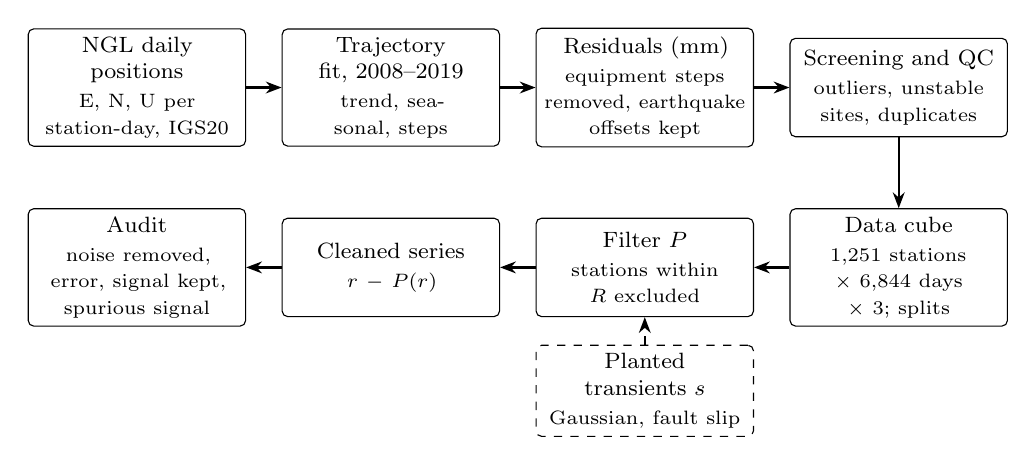
\begin{tikzpicture}[
        box/.style={draw, rounded corners=2pt, align=center, font=\footnotesize, minimum height=1.25cm, text width=2.55cm, inner sep=3pt},
        arr/.style={-{Stealth[length=2mm]}, thick},
      node distance=0.45cm]
      \node[box] (raw) {NGL daily positions\\[1pt]{\scriptsize E, N, U per station-day, IGS20}};
      \node[box, right=of raw] (traj) {Trajectory fit, 2008--2019\\[1pt]{\scriptsize trend, seasonal, steps}};
      \node[box, right=of traj] (res) {Residuals (mm)\\[1pt]{\scriptsize equipment steps removed, earthquake offsets kept}};
      \node[box, right=of res] (qc) {Screening and QC\\[1pt]{\scriptsize outliers, unstable sites, duplicates}};
      \node[box, below=0.9cm of qc] (cube) {Data cube\\[1pt]{\scriptsize 1,251 stations $\times$ 6,844 days $\times$ 3; splits}};
      \node[box, left=of cube] (filt) {Filter $P$\\[1pt]{\scriptsize stations within $R$ excluded}};
      \node[box, left=of filt] (clean) {Cleaned series\\[1pt]{\scriptsize $r - P(r)$}};
      \node[box, left=of clean] (audit) {Audit\\[1pt]{\scriptsize noise removed, error, signal kept, spurious signal}};
      \node[box, below=0.35cm of filt, minimum height=0.8cm, dashed] (plant) {Planted transients $s$\\[1pt]{\scriptsize Gaussian, fault slip}};
      \draw[arr] (raw) -- (traj); \draw[arr] (traj) -- (res); \draw[arr] (res) -- (qc); \draw[arr] (qc) -- (cube);
      \draw[arr] (cube) -- (filt); \draw[arr] (filt) -- (clean); \draw[arr] (clean) -- (audit);
      \draw[arr, dashed] (plant) -- (filt);
  \end{tikzpicture}}
  \caption{Processing chain from daily GNSS positions to the signal-loss audit.}
  \label{fig:pipeline}
\end{figure}

\subsection{Data}
\label{sec:stations}

The data are the daily IGS20 solutions of the Nevada Geodetic Laboratory (NGL) \citep{blewitt2018, ngl2026}. Each solution gives the east, north and up position of a station's antenna relative to a fixed reference point near the station, estimated from 24~hours of observations, with formal uncertainties of about 1~mm in the horizontal and 3--4~mm in the vertical. NGL publishes new days with a latency of about ten days. In southern California the noise in these series contains flicker and random-walk components in addition to white noise \citep{langbein2008}.

All stations between $32.4^\circ$ and $42.1^\circ$N and between $124.6^\circ$ and $114.0^\circ$W with at least 1,095 daily solutions were taken: 1,381 stations in California and adjacent parts of Nevada, Oregon and Baja California. The analysis starts on 1 January 2008. About 390 stations reported on a typical day in 2005, and between about 820 and 1,030 have done so since 2008. Of the 1,381 stations, 130 were removed: 30 with less than one year of data after 2008; 22 with non-tectonic site motion, such as groundwater-driven subsidence in the Central Valley, identified by a robust scale of the trajectory residual (Section~\ref{sec:residuals}) above 10~mm in the horizontal or 30~mm in the vertical; and 78 co-located duplicates within 1~km of a longer-running station, of which only the station with the most data was kept. The remaining 1,251 stations (Fig.~\ref{fig:network}) give $6.45 \times 10^6$ station-days. On 1 July 2018 the median distance to the nearest station was 9.7~km, and a typical station had 22 stations within 50~km and 73 within 100~km. The 16th-nearest neighbour of a station lies at a median distance of 40~km (10th--90th percentiles 22--79~km), the 64th at 88~km and the 256th at 204~km.

\begin{figure}[t]
  \centering
  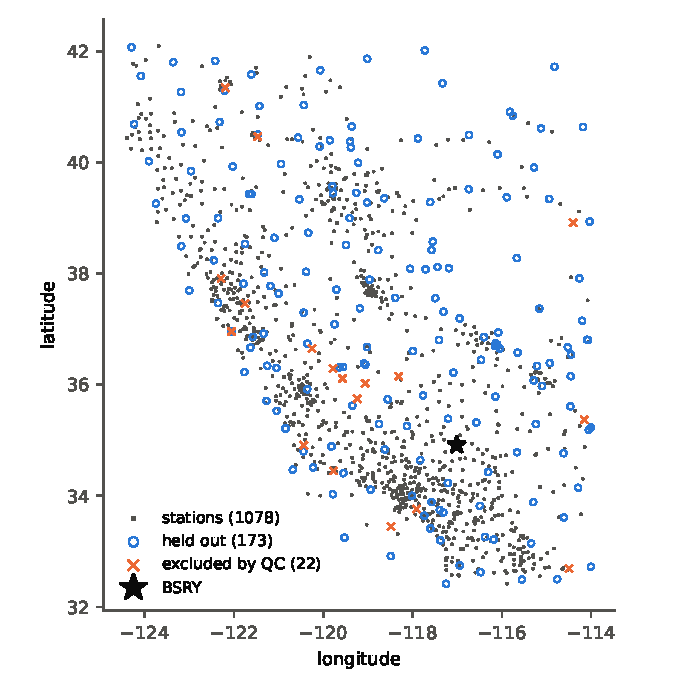
\includegraphics[width=0.7\textwidth]{network_map.pdf}
  \caption{Stations used, held out and excluded.}
  \label{fig:network}
\end{figure}

\subsection{Residuals}
\label{sec:residuals}

For each station $i$ and component $c$, the trajectory model
\begin{equation}
  x_{i,c}(t) = a + v\,(t - t_0) + \sum_{k=1}^{2}\left[p_k \sin(2\pi k t) + q_k \cos(2\pi k t)\right] + \sum_{j} b_j\, H(t - t_j) + r_{i,c}(t)
  \label{eq:trajectory}
\end{equation}
is fitted by least squares, where $a$ is a constant, $v$ a linear rate about the mean epoch $t_0$ of the fitted data, $p_k$ and $q_k$ the amplitudes of the annual and semi-annual harmonics, $b_j$ the amplitudes of Heaviside steps $H$ at the epochs $t_j$ of the NGL step catalogue, $r_{i,c}(t)$ the residual and $t$ the time in years (Fig.~\ref{fig:processing}). Only training days (2008--2019, outside the Ridgecrest exclusion described below) enter the fit, and the fitted trajectory is extrapolated to later years. Equipment steps are removed everywhere: within the training years they are estimated in the fit, and after them by a local estimate, the median residual over the 30 days after the change minus that over the 30 days before. Earthquake steps are not removed from the residuals; those within the training years are estimated in the fit, so that they do not bias the rate, and then added back. A station with fewer than 365 training epochs is fitted on its first 730 days, or its first 365 epochs, whichever reaches further, and is held out (Section~\ref{sec:heldout}).

\begin{figure}[t]
  \centering
  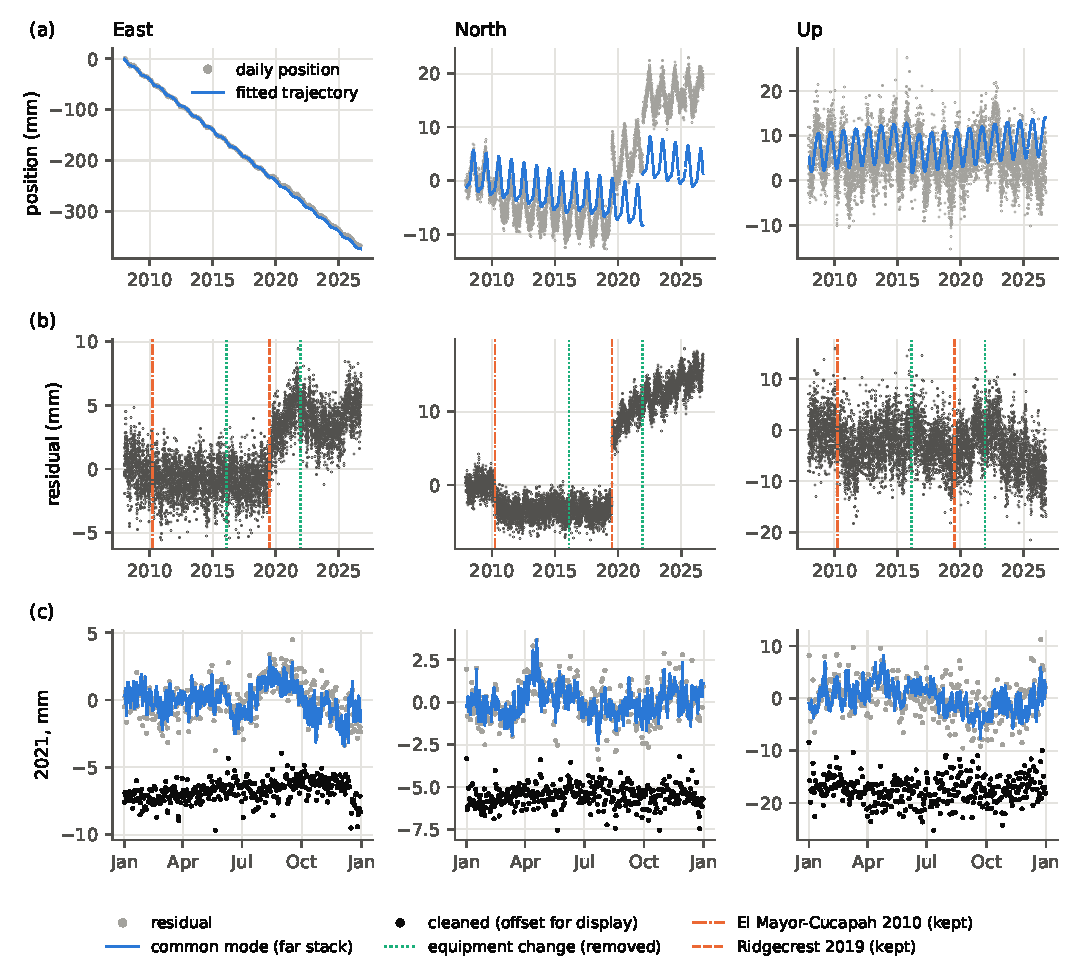
\includegraphics[width=\textwidth]{data_processing.pdf}
  \caption{From positions to residuals at station BSRY: (a) positions and fitted trajectory, (b) residual, (c) one validation year with the network common mode and the cleaned series.}
  \label{fig:processing}
\end{figure}

A value more than five robust standard deviations (1.4826 times the median absolute deviation) from its 61-day running median in any component is treated as missing; 32,544 station-days, about 0.5\% of the data, are removed this way. The station QC of Section~\ref{sec:stations} uses a second trajectory fit from which earthquake steps are also removed, so that coseismic motion does not count against a station. Stations that develop problems after the training years are kept as inputs but not scored: those whose day-to-day scatter increases more than threefold, and those with a jump of more than 50~mm in the horizontal or 100~mm in the vertical between consecutive 30-day medians with no catalogued step within 45 days; 19 stations are excluded from scoring this way. The local equipment-step estimate and the outlier screening use days from every year, including the validation and test years, but no other station; their effect on a day that is kept is at most a constant shift or the removal of a spike.

The residuals, their formal uncertainties and an availability mask are stored in an array of 1,251 stations by 6,844 days by three components, together with the neighbour lists of every station at each exclusion radius (the 16 nearest stations beyond $R$, searched to $R + 300$~km). Days are split into training (2008--2019), validation (2020--2021) and test years (2022 to 26 September 2026, the last day available when the method was frozen); days published after the freeze will form a prospective test.

\subsection{Held-out stations and excluded intervals}
\label{sec:heldout}

The held-out stations are never used in training, and serve to test how well trained filters generalise to stations they have not seen. 125 stations, 10\% of the network, are chosen by farthest-point sampling \citep{gonzalez1985} with seed 0, which starts from a random station and repeatedly adds the station farthest from all those already chosen. A further 56 stations are held out because they have fewer than 365 daily solutions in 2008--2019; 8 stations are in both groups, giving 173 held-out stations. The interval from 1 July 2019 to 30 June 2020 at stations within 150~km of the 2019 Ridgecrest mainshock ($35.77^\circ$N, $117.60^\circ$W) is excluded from training, so that no model is fitted or trained on its postseismic signal.

\subsection{Displacement rather than increments}

Filters are applied to displacement rather than to daily increments. For example, 2~cm of postseismic displacement accumulated over a year is a daily increment of about 0.055~mm, whereas the day-to-day scatter of the increments is about 1.4~mm in the horizontal components. Increments are used only as an additional input to the attention network (Section~\ref{sec:filters-learned}).

%% ===========================================================================
\section{The signal-loss audit}
\label{sec:audit}
%% ===========================================================================

\subsection{Leave-one-out filtering and the exclusion radius}
\label{sec:loo}

A filter $P$ estimates the part of the residual of station $i$ that is shared with other stations, and the cleaned series is $r - P(r)$. A leave-one-out filter never reads station $i$ itself when estimating it, and never reads any station within $R$~km of it (Fig.~\ref{fig:radius}). The target-inclusive filters of Section~\ref{sec:filters-inclusive} read the target on purpose, as published filters of their kind do; they are applied to the same cube and scored on noise removed and on the signal measures, but not on reconstruction error. The exclusion radius $R$ is an experimental variable: M1 is run at $R = 0$, 10, 25, 50, 100, 200 and 400~km and the far stack at 0, 25, 50, 100, 200, 400 and 600~km; the other leave-one-out filters are run at the radii in Table~\ref{tab:radii}, and M2, M3 and M4 at $R = 0$ only.

\begin{figure}[t]
  \centering
  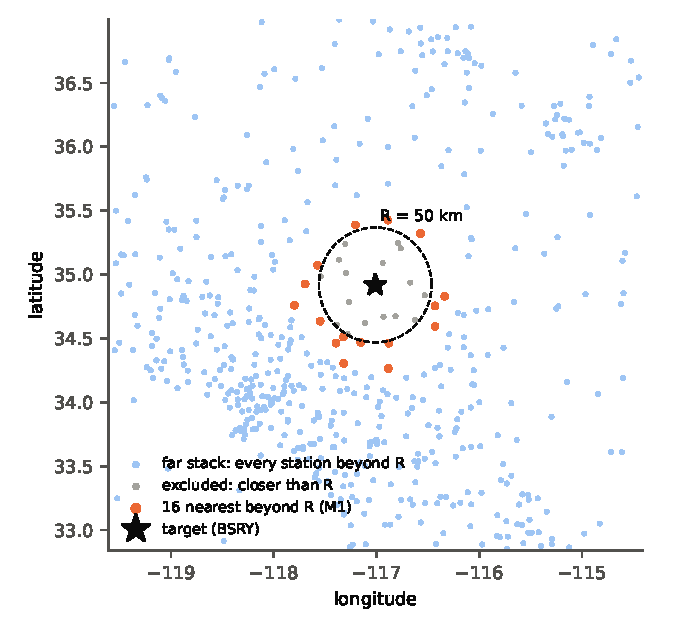
\includegraphics[width=0.7\textwidth]{network_radius.pdf}
  \caption{What a prediction for one target may use at $R = 50$~km.}
  \label{fig:radius}
\end{figure}

Two leak checks are run for every leave-one-out filter at every radius, on the first year of the validation period. Both compare predictions on two inputs that differ only in values the filter must not read. In the radius check, the target and every station within $R$ of it are set to a poison value of $10^6$~mm, for five randomly chosen targets. In the mask check, the cells hidden for the mask scores below are filled once with missing values and once with the poison value, while remaining marked as unavailable. In both, the predictions must agree to within 0.001~mm. Every filter passed both checks at every radius with a largest difference of 0.0~mm. Because a filter that passes the radius check never reads the target, one prediction on the unhidden cube is a leave-one-out prediction for every station at once, and this is how all cleaned series are produced.

The harness also computes scores on fixed evaluation masks (seed 20260101): 10\% of available station-days at random (\texttt{scatter}), one 30-day block per station and year (\texttt{block}), all days of the held-out stations (\texttt{station}) and the Ridgecrest window. These mask scores are not the reconstruction error of Section~\ref{sec:measures}; they are used here only for the spread between training seeds (Section~\ref{sec:res-learned}), and are labelled as such.

\subsection{Measures of noise removed and of planted transients}
\label{sec:measures}

Filters are compared on two measures of noise and two of signal, with a third, velocity repeatability, reported separately. Noise removed is the reduction in short-period scatter at each scored station,
\begin{equation}
  1 - \frac{\mathrm{rms}\big(\mathrm{fast}(r - P(r))\big)}{\mathrm{rms}\big(\mathrm{fast}(r)\big)},
  \label{eq:noise}
\end{equation}
where the fast part of a series is the series minus its 61-day running median. It is averaged over the three components and summarised by its median over stations. Predicting zero gives 0.

Reconstruction error is the root mean square of the fast part of the leave-one-out error $r - P(r)$, normalised by each station's robust noise scale from the training years, averaged over the three components, and summarised by its median over the seen, scored stations. Days within $\pm 30$ days of an M $\ge$ 6 earthquake catalogued for a station are left out. Predicting zero gives 0.753 on the test years and 0.723 on the validation years rather than 1, because separating the slow part also removes some of each station's own noise. Reconstruction error is the criterion on which the leave-one-out filters were tuned, on the validation years.

Retention measures the fraction of a planted transient that survives filtering. A transient $s$ is added to the residuals, and both the original and the modified residuals are filtered. The change in the cleaned series and the retention are
\begin{equation}
  \Delta = \big(r + s - P(r+s)\big) - \big(r - P(r)\big),
  \qquad
  \rho = \frac{\langle \Delta,\, s \rangle}{\langle s,\, s \rangle},
  \label{eq:retention}
\end{equation}
with the inner products over the horizontal components, the days of the transient and the scored stations within $2L$ of its centre, where $L$ is its width. Pairing with the unmodified run removes the noise term; for a linear filter, $\rho = \langle s - P(s), s\rangle / \langle s, s \rangle$ exactly. $\rho = 1$ means that the transient is kept, $\rho = 0$ that it is removed, and $\rho > 1$ that the filter adds to it. Retention is summarised by its median over transients.

Spurious signal is the change created where nothing was planted. A Gaussian transient is set to zero beyond $3L$ from its centre (its footprint). At the scored stations outside the footprint whose cleaned series the transient can change, which depend on the filter (stations with a neighbour inside the footprint for the nearest-neighbour filters, stations whose far set includes one for the far stack, every station of the same region for C3, and every station for C1), the peak horizontal amplitude of $\Delta$ is taken as a fraction of the amplitude of the transient, the largest value over these stations is kept, and its median over transients is reported. For fault-slip events, which have no single amplitude, the stations outside are those moved by less than 0.1~mm by the event, and the reference is the event's largest displacement at a scored station.

Velocity repeatability compares the velocity of each cleaned series on 2022--2023 with that on 2024--2025. Each velocity is a MIDAS-style estimate \citep{blewitt2016}: the median of the slopes between all pairs of days exactly 365 days apart within the window, recomputed after removing slopes more than two robust standard deviations from the first median. Pairs that span a catalogued earthquake step or touch a day left out of scoring are skipped, and at least 100 pairs are required. The measure is the median over stations of $|\Delta v|$, the absolute difference between the two velocities, per component. It was defined before the freeze and implemented on 12 October 2026, after it.

\subsection{Planted and real signals}
\label{sec:planted}

Gaussian transients have the form
\begin{equation}
  s(d, t) = A \exp\!\left(-\frac{d^2}{2L^2}\right) g(t)\, \mathbf{u},
  \label{eq:gaussian}
\end{equation}
where $d$ is the distance of a station from the centre, $A$ the amplitude, $L$ the width, $\mathbf{u}$ a horizontal unit vector in a random direction and $g(t)$ the time profile: a raised-cosine rise over $D$ days, a 60-day hold and a raised-cosine fall over $D$ days, after which the transient is zero, so it leaves no permanent offset. $s$ is zero beyond $3L$, and every station in the footprint moves in the same direction. The grid is $A \in \{2, 5, 10\}$~mm, $L \in \{10, 25, 50, 100\}$~km and $D \in \{10, 30, 90\}$~days. Each of the 36 combinations is planted at 20 centres, each at a randomly chosen scored station, giving 720 transients per filter and radius, of which 714--719 have at least one scored station within $2L$. Onsets fall in 300-day slots of the scored period, and the signal is added only on days with data. Many transients share one run of a filter: two share a run only if no station's cleaned series can be changed by both, so the $\Delta$ at every station comes from one transient, and fewer transients fit in a run at larger radii.

Fault-slip events are computed from source models taken from published studies and moved to other faults of the same style in the SCEC Community Fault Model 7.0 \citep{plesch2007, plesch2024cfm}. Fault surfaces (UTM zone 11, NAD27) are triangulated; a patch of the template's length and depth range is placed at a random position along a fault of the same style, with dip within $\pm 15^\circ$ of the template's; slip is tapered to zero over the outer 20\% of the patch (not at the top when it reaches the surface); and east, north and up displacements at every station are computed from triangular dislocations in an elastic half-space with a Poisson's ratio of 0.25 \citep{nikkhoo2015}. Every template value is a range from the full text of its source, drawn per event. Shallow slow slip follows the 2023 Superstition Hills and Imperial fault events \citep{materna2024, vavra2024}: 8--25~km long, from the surface to 2--4~km depth, 8--45~mm of slip, a slip front moving at 0.4--9~km/day with a local rise of 1--8 days. Afterslip follows the 2010 El Mayor--Cucapah earthquake \citep{gonzalezortega2014}: 15--50~km long, from 0--2 to 5--12~km depth, 10--40~cm of slip with a logarithmic time function ($\tau = 17$--34 days), followed for 365 days. Slip is permanent after the event. An event is kept only where at least three scored stations move by more than 1~mm, and two events share a run only if no station moves by more than 0.1~mm in both. Twenty events of each template are planted, the same for every filter. Retention is computed as in Eq.~\eqref{eq:retention} over the stations moving by more than 1~mm, and also per station, with the station's distance from the slipping patch and its side of the fault. On the test years the afterslip events move a median of 28.5 scored stations by more than 1~mm, with a median largest displacement of 14.3~mm; the shallow slow-slip events move a median of 3.5 stations, with 4.6~mm. A third template, shallow creep triggered on a neighbouring fault \citep{ramos2020, xu2020}, was dropped because only 1 of 300 random placements moved three or more scored stations by more than 1~mm. The elastic half-space, uniform tapered slip, afterslip without its earthquake and placement on any fault of the right style are the limits of this test.

Real earthquake offsets are every catalogued earthquake step in the scored period at a scored station, with an observed horizontal offset of at least 3~mm and no other catalogued step within 15 days. The offset is the mean position over the 10 days after the earthquake minus that over the 10 days before (at least 5 available days on each side), and the fraction kept is $\langle \text{kept}, \text{observed} \rangle / \langle \text{observed}, \text{observed} \rangle$, with ``kept'' the same difference measured on the cleaned series. On the test years there are 81 such offsets (median 6.8~mm): 54 from the 5 December 2024 M7.0 Cape Mendocino earthquake, 18 from the 20 December 2022 M6.4 Ferndale earthquake, 5 from an M5.6 event on 24 June 2026 and 2 each from two M5.7 events (9 December 2024 and 14 April 2026; catalogue identifiers nn00888580 and nn00914068). These offsets have no ground truth, since the observed offset includes noise.

The Ridgecrest test uses the real postseismic displacement after the 6 July 2019 mainshock: at the 182 scored stations within 80~km, the horizontal displacement over days 7--365 relative to the mean of days 1--6 is compared with the same quantity in the cleaned series, as $\langle \text{kept}, \text{observed} \rangle / \langle \text{observed}, \text{observed} \rangle$ per station, and the median over stations is reported. These days are excluded from training, and 2019 is in neither the validation nor the test years, so the result is the same for every period. Figure~\ref{fig:audit} illustrates the measurement of signal kept at one station.

\begin{figure}[t]
  \centering
  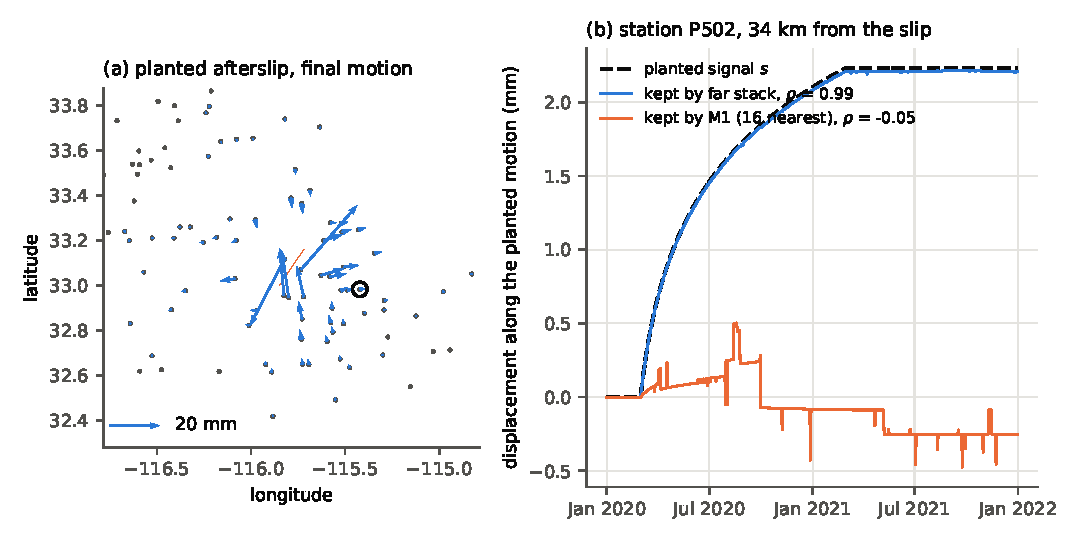
\includegraphics[width=\textwidth]{audit.pdf}
  \caption{Measuring signal kept, at station P502, the median station among the 17 at 15--40~km from a planted afterslip patch (validation years).}
  \label{fig:audit}
\end{figure}

\subsection{Protocol}
\label{sec:protocol}

All design decisions, hyper-parameters and model choices were made on the validation years. The method was frozen on 11 October 2026 (repository tag \texttt{freeze-2026-10-11}), and the results below are from the test years unless marked otherwise. The test years are not untouched: they were looked at while the scoring rules were being revised on 7 October 2026. The untouched evaluation will be the prospective one, once NGL has published a year of days after the freeze. After the freeze, three additions were made without changing the data, filters or scoring rules: velocity repeatability (defined before the freeze and implemented on 12 October), the split of the bootstrap comparison by seen and held-out stations (12 October), and the figure code. The attention network was also run at further radii, and further training seeds were run, as allowed by the freeze rules.

Differences in reconstruction error are tested with a paired block bootstrap (\texttt{gnssdl bench compare}): each station's leave-one-out fast error is summarised per 30-day block, and blocks (the same for every station) and stations are resampled 1,000 times to give a 95\% interval for the difference in the median, run separately for seen stations, held-out stations and all stations. Differences in retention are tested by resampling the planted transients, paired by identifier, for each width. A difference whose interval includes zero is reported as not distinguishable. Trained filters were run with five seeds.

%% ===========================================================================
\section{Filters}
\label{sec:filters}
%% ===========================================================================

Table~\ref{tab:filters} lists the filters. They fall into the three families of Section~\ref{sec:intro}; the learned filters belong to the leave-one-out family but are described separately. No leave-one-out filter reads the target's own values on any day. The ``days used'' column gives the days of the other stations that a prediction for day $t$ reads.

\begin{table}[t]
  \centering
  \small
  \caption{Filters audited. Parameters: learned or tuned parameters at $R = 0$. Days used: days of other stations read by a prediction for day $t$.}
  \label{tab:filters}
  \begin{tabular}{p{1.7cm}p{5.7cm}p{2.2cm}r}
    \toprule
    Name & Description & Days used & Parameters \\
    \midrule
    \multicolumn{4}{l}{\textit{Target-inclusive}} \\
    C1 & Mean of the whole network, target included & $t$ & 0 \\
    C3 & Sub-regional probabilistic PCA; 1, 4 or 8 regions $\times$ 1--3 components & $t$ & $\sim$3.7k/comp. \\
    M2-self & Robust weighted median of the 16 nearest and the target & $t$ (screening: 31 d) & 2 \\
    \multicolumn{4}{l}{\textit{Distance-excluded}} \\
    Far stack & Mean of every station beyond $R$; D1 at $R = 400$~km & $t$ & 0 \\
    \multicolumn{4}{l}{\textit{Leave-one-out over nearest neighbours}} \\
    M1 & Distance-weighted mean of the 16 (64, 256) nearest beyond $R$ & $t$ & 1 \\
    M2 & Robust weighted median of the 16 nearest beyond $R$ & $t$ (screening: 31 d) & 2 \\
    M3a / M3b & Ridge regression on 16 neighbours, per station / pooled & $t$ & 65/station; 257 \\
    M4a / M4b & M3 per period band (under 7, 7--60, 60--400, over 400 days) & all, two-sided & $4 \times$ M3 \\
    \multicolumn{4}{l}{\textit{Learned}} \\
    M3k & Learned kernel: neighbour weight from distance, azimuth and noise level; 16 or 256 neighbours & $t$ & 1,411 \\
    M5 & Space--time attention: 32 neighbours and the far stack, 64-day window, correction to the far stack & 64-day windows, two-sided & 212,048 \\
    M5-aug & M5 trained with planted transients in its inputs & as M5 & 212,048 \\
    \bottomrule
  \end{tabular}
\end{table}

\subsection{Target-inclusive filters}
\label{sec:filters-inclusive}

C1 is the stack of \citet{wdowinski1997}: the common mode of every station on a day is the unweighted mean of all available stations that day, the station itself included. C3 is sub-regional probabilistic PCA \citep{tipping1999}, applied as in \citet{gruszczynski2018} with regions as in \citet{liu2026}: stations are grouped into 1, 4 or 8 regions by k-means on their projected coordinates; in each region and component, a probabilistic PCA with 1, 2 or 3 components is fitted by expectation--maximisation on the quiet training residuals (Section~\ref{sec:filters-learned}), normalised per station, with missing days treated as latent; on any day the component scores are estimated from every available station of the region, the target included, and the common mode is the reconstruction. The nine settings are reported as a range, and individually in Table~\ref{tab:c3}. M2-self is the robust weighted median of M2 (Section~\ref{sec:filters-loo}) with the target's own value added to the median, as in CMC Imaging \citep{tianshen2016, kreemer2021}; it reuses M2's tuned settings.

\subsection{Distance-excluded filters}
\label{sec:filters-distance}

The far stack is the unweighted mean of every available station at least $R$ from the target, the target excluded, per day and component. It has no parameters and is run at $R = 0$, 25, 50, 100, 200, 400 and 600~km. D1 is the far stack at $R = 400$~km, the distance of \citet{bachelot2025}, computed separately; its results agree with those of the far stack at 400~km. \citet{bachelot2025} use the eight nearest stations beyond 400~km in a graph neural network and compare it with a stack of the same stations; D1 uses every station beyond 400~km.

\subsection{Leave-one-out filters over nearest neighbours}
\label{sec:filters-loo}

These filters predict the target from its $K$ nearest stations beyond $R$, using only day $t$ (M1--M3) or the neighbours' whole series (M4). Their settings were chosen on the validation years by reconstruction error.

M1 is the weighted mean $\hat r_i(t) = \sum_j w_{ij} a_j(t) r_j(t) / \sum_j w_{ij} a_j(t)$ over the 16 nearest stations, with $w_{ij} = \exp(-d_{ij}^2/2\ell^2)/\bar\sigma_j^2$, $a_j(t)$ the availability and $\bar\sigma_j$ the station's median formal uncertainty over the training years, per component. The length scale $\ell$ was chosen from 10~km to infinity (a plain mean): 50~km at $R = 0$ for 16 and 64 neighbours, and 100~km for 256. M1 with 64 and 256 neighbours forms the neighbour-count experiment.

M2 follows \citet{kreemer2021}: a neighbour's value on day $t$ is dropped if it differs from that neighbour's own 31-day running median by more than $k$ times its robust scale; the rest are combined by a weighted median with M1's weights, interpolated as in \citet{kreemer2021}. With fewer than three neighbours left it falls back to M1. The tuned values at $R = 0$ are $\ell = 200$~km and $k = 5$.

M3 is ridge regression on the three components of the 16 neighbours, an availability bit per neighbour and an intercept, in units of each station's noise scale. Missing neighbours are set to zero and the remaining values rescaled by $K$ divided by the number available, so that gaps do not bias the fit. Rows are replicated four times with neighbours dropped at random. M3a fits one weight vector per station and component (65 features; $\lambda = 0.1$ in units of the trace of the Gram matrix per feature); the 178 stations without enough training rows, the held-out stations among them, use M3b. M3b fits one weight vector per component for all stations, adding each neighbour slot's log distance and azimuth and their products with the slot's residuals (257 features; $\lambda = 0.01$).

M4 applies M3 separately to four period bands that add up exactly to each series (under 7, 7--60, 60--400 and over 400 days), obtained with differences of zero-phase Gaussian smoothers, and sums the four predictions; $\lambda$ is chosen per band. Before filtering, each series' gaps are filled by linear interpolation of its own days, and a neighbour missing on a day contributes zero with its availability bit off. The band filters read the neighbours' past and future days. M4a is per station and M4b pooled, as M3a and M3b.

\subsection{Learned filters}
\label{sec:filters-learned}

M3k and M5 are trained on quiet residuals: the residuals minus the earthquake offsets estimated in the training-years fit, on training days, outside the Ridgecrest exclusion and outside $\pm 30$ days of catalogued M $\ge$ 6 earthquakes, at stations that are not held out. The loss is the squared error in units of each station's robust noise scale. Training stops early on the validation reconstruction error, and each model was trained with five seeds; the reported results are those of seed 0.

M3k keeps M1's form and learns its kernel: $w_{ijc} = \mathrm{softplus}(f_\theta(g_{ij}, q_j))_c$, where $g_{ij}$ is the neighbour's log distance and the sine and cosine of its azimuth from the target, $q_j$ its log robust noise scale per component and record completeness, and $f_\theta$ a multilayer perceptron with two hidden layers of 32 units (1,411 parameters). The weights depend on where a neighbour is and what kind of station it is, never on its values, so once trained M3k is a fixed weighted mean of day $t$. It was trained over 16 and over 256 neighbours at every radius; at $R = 0$ the best epoch was 14 of 20 (16 neighbours) and 4 of 10 (256).

M5 is a space--time attention network. A sample is a target, its 32 nearest stations beyond $R$, chosen for each 64-day window among the 64 nearest by availability, and one summary node, the far stack. Each node has 17 input channels per day: residual, log formal uncertainty, availability, a flag for cells hidden by a training mask, the daily increment $r(t) - r(t-1)$ (zero unless both days exist), the station's log noise scale and record completeness, and the day of year (sine and cosine), all in units of the station's noise scale. A convolution cuts each node's window into 4-day tokens; three blocks then alternate attention over a node's own tokens (time) and attention over the nodes at the same token (space), the latter biased by each node's log distance, azimuth and type relative to the target ($d = 64$, four heads). The output is a correction added to the far stack, so training starts from the far stack. The target is hidden for the whole window, so predictions never read it. Training used batches of 64 samples, a learning rate of $10^{-3}$ with 500 warm-up steps, weight decay $10^{-4}$, dropout 0.1, neighbour dropout 0.3, and early stopping every 500 steps (best step 5,000 at $R = 0$). Prediction uses 64-day windows overlapping by half, combined with a triangular taper, so a day's prediction reads neighbours' days before and after it. M5 was trained at $R = 0$, 10, 25, 50 and 100~km.

M5-aug is the same network trained with planted transients. In half of the training samples a synthetic field is added to the inputs of every node and to the far-stack node as it would enter that mean, but not to the targets, so copying it into a prediction increases the loss. The field is centred at a random point within $R + 300$~km of the target, with a width of 5--150~km, an amplitude of 1--15 times the station's noise scale, a duration of 5--60 days with a raised-cosine rise and fall, and a random horizontal direction; half are Gaussian blobs and half dipoles, whose sign flips across a random line through the centre. The generator uses its own seed and shapes and runs on training days only, so it is separate from the evaluation transients. M5-aug was trained at $R = 0$ and 25~km (best step 1,500 at $R = 0$).

\subsection{Implementation and use of AI tools}
\label{sec:ai}

The \texttt{gnssdl} package, its tests (120 automated tests, including the leak checks), the design documents and the figure code were written by Claude Opus 5.5 (Anthropic) through Claude Code, under the author's direction, between 6 and 13 October 2026. The research questions are the author's. The code is openly available at \url{https://github.com/hogib/gnssdl} under the MIT licence; per-model results, logs and checkpoints are kept in \texttt{data/runs/<model>/}. This report was drafted by the same tool from the repository and its results files.

%% ===========================================================================
\section{Results}
\label{sec:results}
%% ===========================================================================

Table~\ref{tab:results} summarises the results at $R = 0$ on the test years. The subsections give the supporting numbers. Validation-year values are marked (val).

\begin{table}[t]
  \centering
  \small
  \caption{Main results at $R = 0$ unless stated, test years (2022 to September 2026). Error: leave-one-out reconstruction error (lower is better; zero prediction 0.753). Kept: median retention of 25- and 100-km Gaussian transients. Spurious: for 100-km transients. Afterslip: per-station retention at 15--40~km from the patch. Offsets: real earthquake offsets. Ridgecrest: postseismic displacement kept.}
  \label{tab:results}
  \resizebox{\textwidth}{!}{%
    \begin{tabular}{lccccccc}
      \toprule
      Filter & Error & Noise removed & Kept 25 / 100 km & Spurious & Afterslip & Offsets & Ridgecrest \\
      \midrule
      C1 & -- & 22.8\% & 0.98 / 0.83 & 0.12 & 1.00 & 0.88 & 0.91 \\
      C3 (9 settings) & -- & 16.2--23.1\% & 0.86--0.99 / 0.31--0.85 & 0.24--1.58 & 0.97--1.00 & 0.67--0.87 & 0.79--0.94 \\
      M2-self & -- & 19.3\% & 0.24 / 0.00 & 0.11 & 0.18 & 0.14 & 0.33 \\
      Far stack & 0.566 & 22.7\% & 0.98 / 0.83 & 0.12 & 1.00 & 0.88 & 0.92 \\
      D1 ($R = 400$~km) & 0.585 & 20.5\% & 1.00 / 1.00 & 0.25 & 1.00 & 0.91 & 0.91 \\
      M1 & 0.621 & 14.1\% & 0.25 / 0.00 & 0.02 & 0.11 & 0.09 & 0.31 \\
      M1, 64 & 0.596 & 18.0\% & 0.53 / 0.03 & 0.04 & -- & -- & 0.58 \\
      M1, 256 & 0.606 & 17.2\% & 0.84 / 0.20 & 0.11 & 0.96 & 0.45 & 0.84 \\
      M2 & 0.638 & 12.2\% & 0.28 / 0.00 & 0.12 & 0.20 & 0.12 & 0.37 \\
      M3a & 0.603 & 16.6\% & 0.39 / 0.16 & 0.04 & 0.23 & 0.20 & 0.50 \\
      M3b & 0.599 & 15.6\% & 0.30 / 0.07 & 0.04 & 0.24 & 0.21 & 0.50 \\
      M4a & 0.582 & 19.5\% & 0.52 / 0.34 & 0.04 & 0.54 & 0.23 & 0.85 \\
      M4b & 0.598 & 15.9\% & 0.33 / 0.11 & 0.04 & 0.33 & 0.20 & 0.50 \\
      M3k & 0.595 & 18.0\% & 0.25 / 0.01 & 0.03 & 0.13 & 0.22 & 0.36 \\
      M3k, 256 & 0.562 & 22.7\% & 0.70 / 0.20 & 0.18 & 0.72 & 0.61 & 0.76 \\
      M5 & 0.563 & 22.5\% & 0.83 / 0.59 & 0.16 & 0.90 & 0.78 & 0.91 \\
      M5-aug & 0.565 & 22.6\% & 0.98 / 0.82 & 0.16 & 0.99 & 0.88 & 0.91 \\
      \bottomrule
  \end{tabular}}
\end{table}

\subsection{The trade-off between noise removed and signal kept}
\label{sec:res-tradeoff}

Figure~\ref{fig:tradeoff} plots noise removed against retention of 100-km transients for every filter, with the radius sweeps as lines. Table~\ref{tab:radii} gives the sweeps. For the far stack, from $R = 0$ to 400~km, retention of 100-km transients rises from 0.83 to 1.00, spurious signal from 0.12 to 0.25 and reconstruction error from 0.566 to 0.585, and noise removed falls from 22.7\% to 20.5\%; at 600~km noise removed is 17.7\% and spurious signal 0.33. For M1, retention of 100-km transients rises from 0.00 at $R = 0$ to 1.00 at 400~km, spurious signal from 0.02 to 0.78, and noise removed falls from 14.1\% to 4.7\%. For M5, from $R = 0$ to 100~km, retention of 100-km transients rises from 0.59 to 0.83 and noise removed stays between 22.5\% and 22.7\%; spurious signal is 0.14--0.16 throughout. M5-aug at $R = 25$~km keeps 0.98 and 0.83 of 25- and 100-km transients and removes 22.6\%.

\begin{figure}[t]
  \centering
  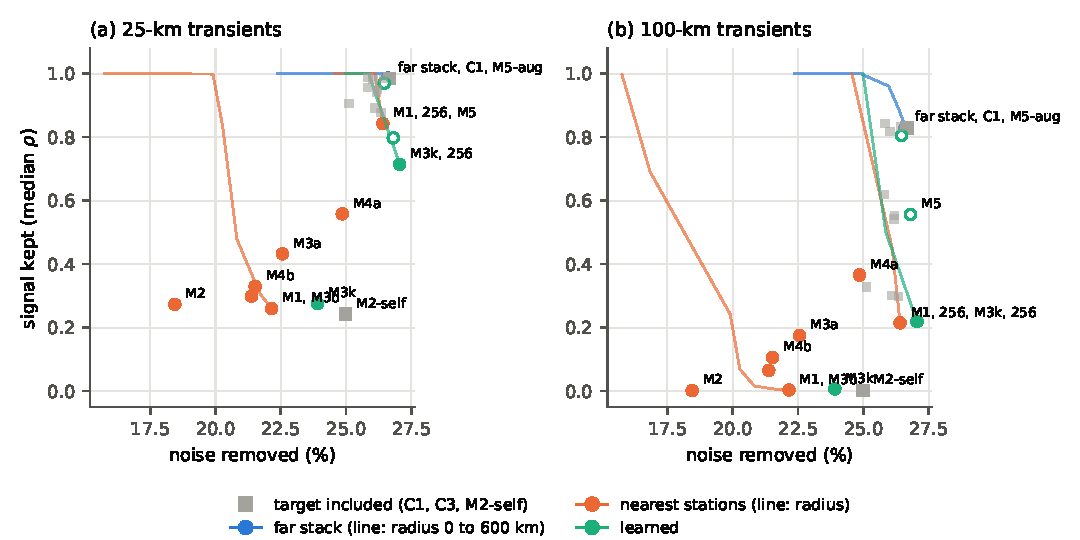
\includegraphics[width=\textwidth]{tradeoff.pdf}
  \caption{Noise removed against retention of 100-km Gaussian transients, test years. Points: filters at $R = 0$; lines: radius sweeps.}
  \label{fig:tradeoff}
\end{figure}

\begin{table}[t]
  \centering
  \small
  \caption{Radius sweeps, test years. Error: leave-one-out reconstruction error (computed for the far stack, M1 and, at $R = 0$, the learned filters). Spurious: 100-km transients.}
  \label{tab:radii}
  \resizebox{\textwidth}{!}{%
  \begin{tabular}{lrcccccc}
    \toprule
    Filter & $R$ (km) & Error & Noise removed & Kept 25 / 100 km & Spurious & Offsets & Ridgecrest \\
    \midrule
    Far stack & 0 & 0.566 & 22.7\% & 0.98 / 0.83 & 0.12 & 0.88 & 0.92 \\
     & 25 & 0.566 & 22.7\% & 0.99 / 0.84 & 0.12 & -- & 0.92 \\
     & 50 & 0.567 & 22.6\% & 1.00 / 0.86 & 0.13 & -- & 0.92 \\
     & 100 & 0.569 & 22.5\% & 1.00 / 0.89 & 0.14 & 0.88 & 0.92 \\
     & 200 & 0.572 & 22.1\% & 1.00 / 0.96 & 0.16 & -- & 0.93 \\
     & 400 & 0.585 & 20.5\% & 1.00 / 1.00 & 0.25 & 0.91 & 0.91 \\
     & 600 & 0.604 & 17.7\% & 1.00 / 1.00 & 0.33 & -- & 0.88 \\
    M1 & 0 & 0.621 & 14.1\% & 0.25 / 0.00 & 0.02 & 0.09 & 0.31 \\
     & 10 & 0.623 & 13.9\% & 0.29 / 0.00 & 0.03 & -- & 0.44 \\
     & 25 & 0.630 & 13.1\% & 0.45 / 0.01 & 0.03 & -- & 0.58 \\
     & 50 & 0.637 & 13.0\% & 0.83 / 0.06 & 0.05 & -- & 0.74 \\
     & 100 & 0.660 & 10.6\% & 1.00 / 0.23 & 0.10 & 0.78 & 0.94 \\
     & 200 & 0.699 & 6.3\% & 1.00 / 0.70 & 0.41 & -- & 0.94 \\
     & 400 & 0.706 & 4.7\% & 1.00 / 1.00 & 0.78 & 0.92 & 0.90 \\
    M1, 64 & 0 & 0.596 & 18.0\% & 0.53 / 0.03 & 0.04 & -- & 0.58 \\
     & 100 & 0.601 & 17.8\% & 1.00 / 0.33 & 0.15 & -- & 0.96 \\
     & 400 & 0.634 & 14.2\% & 1.00 / 1.00 & 0.62 & -- & 0.90 \\
    M1, 256 & 0 & 0.606 & 17.2\% & 0.84 / 0.20 & 0.11 & 0.45 & 0.84 \\
     & 100 & 0.599 & 18.2\% & 1.00 / 0.44 & 0.19 & 0.82 & 0.92 \\
     & 400 & 0.597 & 18.5\% & 1.00 / 1.00 & 0.44 & 0.90 & 0.93 \\
    M3k & 0 & 0.595 & 18.0\% & 0.25 / 0.01 & 0.03 & 0.22 & 0.36 \\
     & 100 & -- & 16.2\% & 1.00 / 0.24 & 0.10 & 0.77 & 0.99 \\
     & 400 & -- & 12.2\% & 1.00 / 1.00 & 0.79 & 0.92 & 0.93 \\
    M3k, 256 & 0 & 0.562 & 22.7\% & 0.70 / 0.20 & 0.18 & 0.61 & 0.76 \\
     & 100 & -- & 20.1\% & 1.00 / 0.49 & 0.27 & 0.79 & 0.94 \\
     & 400 & -- & 21.1\% & 1.00 / 1.00 & 0.48 & 0.90 & 0.93 \\
    M5 & 0 & 0.563 & 22.5\% & 0.83 / 0.59 & 0.16 & 0.78 & 0.91 \\
     & 10 & -- & 22.7\% & 0.95 / 0.75 & 0.14 & 0.84 & 0.91 \\
     & 25 & -- & 22.6\% & 0.96 / 0.76 & 0.14 & 0.84 & 0.91 \\
     & 50 & -- & 22.6\% & 0.99 / 0.81 & 0.14 & 0.86 & 0.90 \\
     & 100 & -- & 22.5\% & 1.00 / 0.83 & 0.15 & 0.88 & 0.91 \\
    M5-aug & 0 & 0.565 & 22.6\% & 0.98 / 0.82 & 0.16 & 0.88 & 0.91 \\
     & 25 & -- & 22.6\% & 0.98 / 0.83 & 0.17 & 0.88 & 0.91 \\
    \bottomrule
  \end{tabular}}
\end{table}

\subsection{Number of stations versus distance}
\label{sec:res-count}

Figure~\ref{fig:count} compares filters that differ in the number of stations they average. At $R = 0$ on the test years, the reconstruction error is 0.621 for M1 over 16 neighbours, 0.596 over 64, 0.606 over 256 and 0.566 for the far stack, which averages all 1,250 other stations; on the validation years the same four values are 0.531, 0.511, 0.507 and 0.509 (val). Noise removed on the test years is 14.1\%, 18.0\%, 17.2\% and 22.7\%. Retention of 25-km transients is 0.25, 0.53, 0.84 and 0.98, and of 100-km transients 0.00, 0.03, 0.20 and 0.83. At $R = 100$~km the reconstruction errors are 0.660 (16), 0.601 (64), 0.599 (256) and 0.569 (far stack).

\begin{figure}[t]
  \centering
  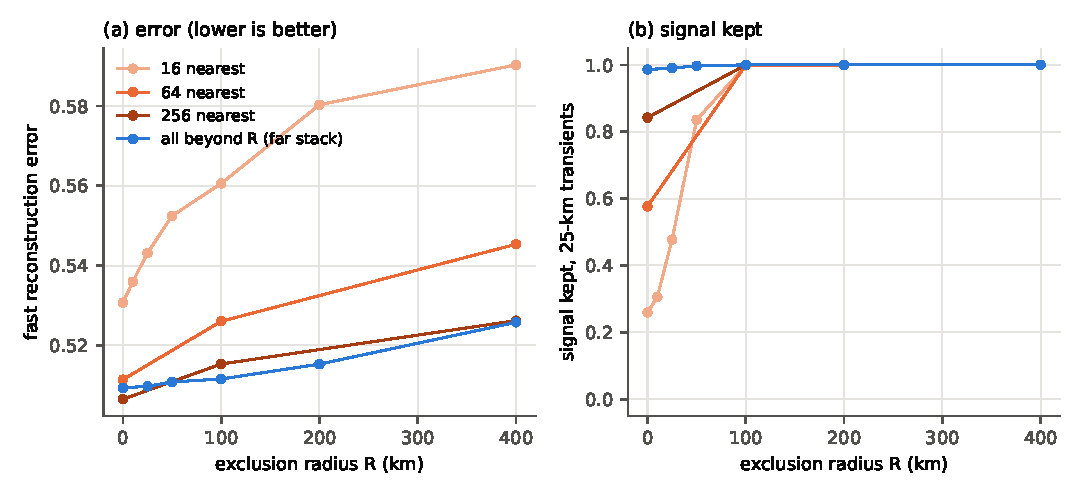
\includegraphics[width=\textwidth]{count_vs_distance.pdf}
  \caption{Reconstruction error (a) and retention of 25-km transients (b) against exclusion radius for M1 over 16, 64 and 256 neighbours and the far stack, test years.}
  \label{fig:count}
\end{figure}

Regression on the same 16 neighbours gives reconstruction errors of 0.603 (M3a), 0.599 (M3b), 0.582 (M4a) and 0.598 (M4b), against 0.621 for M1; noise removed is 16.6\%, 15.6\%, 19.5\% and 15.9\%. Retention of 25- and 100-km transients is 0.39 and 0.16 (M3a), 0.30 and 0.07 (M3b), 0.52 and 0.34 (M4a) and 0.33 and 0.11 (M4b), against 0.25 and 0.00 for M1. On the validation years the per-station regressions had lower errors than the pooled ones (M3a 0.527, M3b 0.534; M4a 0.517, M4b 0.532; val); on the test years M3a's error is higher than M3b's.

\subsection{Retention by width, amplitude and duration}
\label{sec:res-grid}

Table~\ref{tab:width} gives retention for each width. Across the three amplitudes (2, 5 and 10~mm), median retention of a given width changes by at most 0.15 for any filter (M3k at 25~km: 0.20, 0.35 and 0.25); for M1 at 25~km it is 0.20, 0.30 and 0.25, for the far stack at 100~km 0.85, 0.82 and 0.83, and for M5 at 100~km 0.57, 0.58 and 0.63. Across the three durations (10, 30 and 90 days) it changes by at most 0.20 (C3 with four regions and three components at 100~km: 0.54, 0.41 and 0.61); for the far stack at 100~km it is 0.83, 0.81 and 0.86, and for M4a at 100~km 0.29, 0.33 and 0.41. Spurious signal for 10-km transients is 0.20 for M1, 0.50 for M2 and 0.43 for M2-self, against 0.00 for the far stack; for 100-km transients it is 0.02, 0.12, 0.11 and 0.12 (Table~\ref{tab:width}).

\begin{table}[t]
  \centering
  \small
  \caption{Median retention and spurious signal of Gaussian transients by width $L$, $R = 0$, test years.}
  \label{tab:width}
  \resizebox{\textwidth}{!}{%
  \begin{tabular}{lcccccccc}
    \toprule
     & \multicolumn{4}{c}{Retention} & \multicolumn{4}{c}{Spurious signal} \\
    \cmidrule(lr){2-5}\cmidrule(lr){6-9}
    Filter & 10 & 25 & 50 & 100~km & 10 & 25 & 50 & 100~km \\
    \midrule
    C1 & 1.00 & 0.98 & 0.94 & 0.83 & 0.00 & 0.01 & 0.04 & 0.12 \\
    M2-self & 0.75 & 0.24 & 0.03 & 0.00 & 0.43 & 0.31 & 0.17 & 0.11 \\
    Far stack & 1.00 & 0.98 & 0.94 & 0.83 & 0.00 & 0.01 & 0.04 & 0.12 \\
    D1 & 1.00 & 1.00 & 1.00 & 1.00 & 0.01 & 0.04 & 0.11 & 0.25 \\
    M1 & 0.77 & 0.25 & 0.05 & 0.00 & 0.20 & 0.12 & 0.06 & 0.02 \\
    M1, 64 & 0.90 & 0.53 & 0.18 & 0.03 & 0.11 & 0.18 & 0.10 & 0.04 \\
    M1, 256 & 0.97 & 0.84 & 0.52 & 0.20 & 0.03 & 0.13 & 0.22 & 0.11 \\
    M2 & 0.82 & 0.28 & 0.04 & 0.00 & 0.50 & 0.33 & 0.19 & 0.12 \\
    M3a & 0.83 & 0.39 & 0.21 & 0.16 & 0.20 & 0.13 & 0.06 & 0.04 \\
    M3b & 0.78 & 0.30 & 0.11 & 0.07 & 0.21 & 0.16 & 0.07 & 0.04 \\
    M4a & 0.88 & 0.52 & 0.39 & 0.34 & 0.17 & 0.12 & 0.06 & 0.04 \\
    M4b & 0.78 & 0.33 & 0.16 & 0.11 & 0.20 & 0.14 & 0.07 & 0.04 \\
    M3k & 0.77 & 0.25 & 0.04 & 0.01 & 0.22 & 0.15 & 0.06 & 0.03 \\
    M3k, 256 & 0.88 & 0.70 & 0.45 & 0.20 & 0.05 & 0.09 & 0.22 & 0.18 \\
    M5 & 0.95 & 0.83 & 0.72 & 0.59 & 0.08 & 0.09 & 0.09 & 0.16 \\
    M5-aug & 1.00 & 0.98 & 0.93 & 0.82 & 0.02 & 0.03 & 0.07 & 0.16 \\
    \bottomrule
  \end{tabular}}
\end{table}

\subsection{Sub-regional PCA settings}
\label{sec:res-c3}

Table~\ref{tab:c3} gives the nine C3 settings. With one region, retention of 100-km transients is 0.81--0.85 and spurious signal 0.57--1.58, the largest value being for one component. With eight regions, retention of 100-km transients is 0.31--0.35 and spurious signal 0.24--0.29.

\begin{table}[t]
  \centering
  \small
  \caption{C3 settings ($k$ regions, $p$ components), $R = 0$, test years.}
  \label{tab:c3}
  \resizebox{\textwidth}{!}{%
  \begin{tabular}{lcccccc}
    \toprule
    Setting & Noise removed & Kept 25 / 100 km & Spurious & Afterslip & Offsets & Ridgecrest \\
    \midrule
    $k = 1$, $p = 1$ & 22.7\% & 0.99 / 0.85 & 1.58 & 1.00 & 0.87 & 0.92 \\
    $k = 1$, $p = 2$ & 23.1\% & 0.98 / 0.82 & 0.58 & 1.00 & 0.87 & 0.92 \\
    $k = 1$, $p = 3$ & 21.9\% & 0.98 / 0.81 & 0.57 & 1.00 & 0.87 & 0.92 \\
    $k = 4$, $p = 1$ & 19.8\% & 0.95 / 0.58 & 0.39 & 0.99 & 0.82 & 0.94 \\
    $k = 4$, $p = 2$ & 19.5\% & 0.94 / 0.56 & 0.43 & 0.99 & 0.78 & 0.94 \\
    $k = 4$, $p = 3$ & 19.0\% & 0.93 / 0.54 & 0.46 & 0.99 & 0.78 & 0.93 \\
    $k = 8$, $p = 1$ & 16.2\% & 0.90 / 0.35 & 0.24 & 0.99 & 0.68 & 0.84 \\
    $k = 8$, $p = 2$ & 19.1\% & 0.88 / 0.32 & 0.28 & 0.97 & 0.67 & 0.83 \\
    $k = 8$, $p = 3$ & 19.1\% & 0.86 / 0.31 & 0.29 & 0.97 & 0.69 & 0.79 \\
    \bottomrule
  \end{tabular}}
\end{table}

\subsection{Realistic transients}
\label{sec:res-events}

Figure~\ref{fig:distance} and Table~\ref{tab:afterslip} give afterslip retention per station against distance from the slipping patch. Within 5~km every filter keeps 0.94--1.01. At 15--40~km retention is 0.11 (M1), 0.13 (M3k), 0.20 (M2), 0.18 (M2-self), 0.23 (M3a), 0.24 (M3b), 0.33 (M4b), 0.54 (M4a), 0.72 (M3k-256), 0.90 (M5), 0.96 (M1-256), 0.99 (M5-aug) and 1.00 (far stack, C1, D1). Beyond 40~km it is $-0.05$ (M1), $-0.05$ (M3k), 0.41 (M4a), 0.47 (M3k-256), 0.75 (M1-256), 0.77 (M5), 0.97 (M5-aug) and 0.98 (far stack). Within 15~km of the patch, the two sides of the fault differ by up to 0.11 (M3a 0.99 and 0.88; M3k 0.94 and 0.83; M1 0.95 and 0.88), and by at most 0.02 for the far stack, C1, M5 and M5-aug. Retention over the whole event, over all stations moving by more than 1~mm, is 0.79--1.00 for every filter (lowest M2-self 0.79, M2 0.86, M3k 0.86, M1 0.87).

\begin{figure}[t]
  \centering
  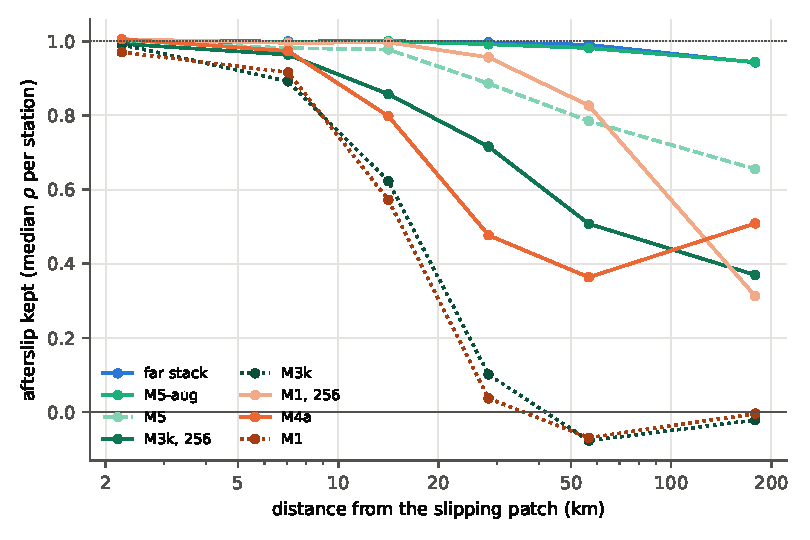
\includegraphics[width=0.8\textwidth]{distance_from_fault.pdf}
  \caption{Afterslip kept per station against distance from the slipping patch, $R = 0$, test years.}
  \label{fig:distance}
\end{figure}

\begin{table}[t]
  \centering
  \small
  \caption{Afterslip retention per station by distance from the slipping patch (median), and the shallow slow-slip events, $R = 0$, test years.}
  \label{tab:afterslip}
  \begin{tabular}{lcccccc}
    \toprule
     & \multicolumn{4}{c}{Afterslip, distance from patch} & \multicolumn{2}{c}{Shallow slow slip} \\
    \cmidrule(lr){2-5}\cmidrule(lr){6-7}
    Filter & 0--5 & 5--15 & 15--40 & over 40~km & Kept & Spurious \\
    \midrule
    C1 & 1.00 & 1.00 & 1.00 & 0.98 & 1.00 & 0.00 \\
    M2-self & 0.94 & 0.78 & 0.18 & $-0.04$ & 0.98 & 0.21 \\
    Far stack & 1.00 & 1.00 & 1.00 & 0.98 & 1.00 & 0.00 \\
    D1 & 1.00 & 1.00 & 1.00 & 1.00 & 1.00 & 0.00 \\
    M1 & 0.97 & 0.89 & 0.11 & $-0.05$ & 1.00 & 0.09 \\
    M1, 256 & 1.01 & 1.00 & 0.96 & 0.75 & 1.00 & 0.01 \\
    M2 & 0.96 & 0.85 & 0.20 & $-0.04$ & 0.99 & 0.27 \\
    M3a & 0.99 & 0.89 & 0.23 & 0.06 & 0.99 & 0.09 \\
    M3b & 0.97 & 0.89 & 0.24 & 0.08 & 0.99 & 0.07 \\
    M4a & 1.01 & 0.96 & 0.54 & 0.41 & 1.00 & 0.09 \\
    M4b & 0.96 & 0.86 & 0.33 & 0.19 & 0.99 & 0.08 \\
    M3k & 0.99 & 0.85 & 0.13 & $-0.05$ & 0.97 & 0.08 \\
    M3k, 256 & 0.99 & 0.94 & 0.72 & 0.47 & 0.97 & 0.02 \\
    M5 & 1.00 & 0.98 & 0.90 & 0.77 & 0.99 & 0.03 \\
    M5-aug & 1.00 & 1.00 & 0.99 & 0.97 & 1.00 & 0.01 \\
    \bottomrule
  \end{tabular}
\end{table}

The shallow slow-slip events are kept by every filter (0.97--1.00 over the whole event). The spurious signal they create, as a fraction of the event's largest displacement, is 0.27 for M2, 0.21 for M2-self, 0.07--0.09 for M1, M3 and M4, 0.08 for M3k, 0.03 for M5 and 0.00 for the far stack and C1 (Table~\ref{tab:afterslip}).

\subsection{Real earthquake offsets and Ridgecrest}
\label{sec:res-real}

The fraction of the 81 real offsets kept is 0.88 for the far stack, C1 and M5-aug, 0.91 for D1, 0.78 for M5, 0.61 for M3k-256, 0.45 for M1-256, 0.20--0.23 for M3, M4 and M3k, 0.14 for M2-self, 0.12 for M2 and 0.09 for M1 (Table~\ref{tab:results}). On the validation years, with 37 offsets mainly from the 2020 Monte Cristo Range, 2021 Antelope Valley and 2021 Petrolia earthquakes, the fraction kept was 0.98 for the far stack, 0.99 for D1, 0.98 for M5-aug, 0.88 for M5 and 0.72 for M1 (val). Of the Ridgecrest postseismic displacement, the far stack keeps 0.92, C1, D1, M5 and M5-aug 0.91, M4a 0.85, M1-256 0.84, M3k-256 0.76, M3a, M3b and M4b 0.50, M2 0.37, M3k 0.36, M2-self 0.33 and M1 0.31. Figure~\ref{fig:real} plots both against retention of 25-km Gaussian transients; the Spearman rank correlation over the fifteen filters is 0.91 for the offsets and 0.93 for Ridgecrest (0.94 and 0.92 on the validation years).

\begin{figure}[t]
  \centering
  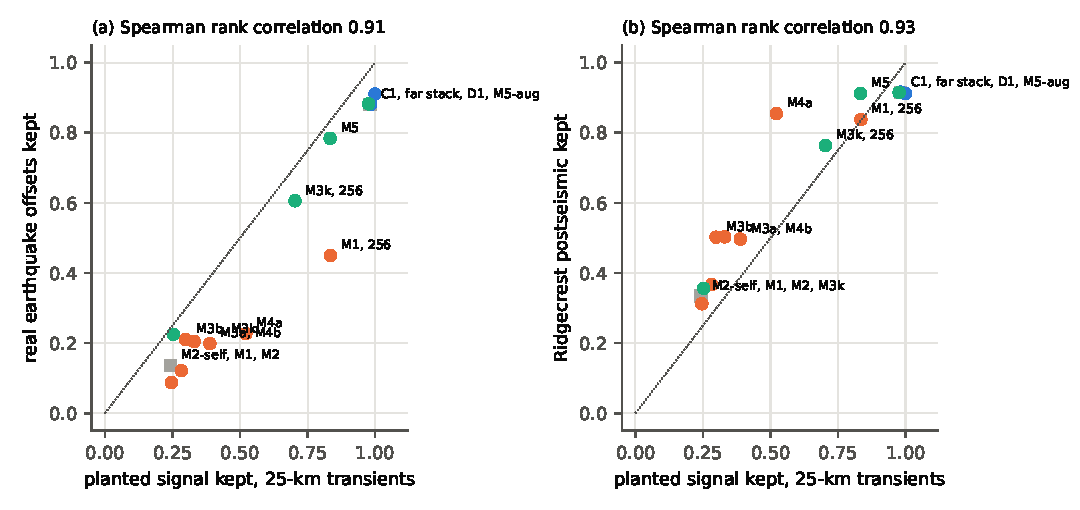
\includegraphics[width=\textwidth]{planted_vs_real.pdf}
  \caption{Real earthquake offsets (a) and Ridgecrest postseismic displacement (b) kept, against retention of 25-km Gaussian transients, $R = 0$, test years.}
  \label{fig:real}
\end{figure}

\subsection{Learned models}
\label{sec:res-learned}

Over 16 neighbours, M3k has a reconstruction error of 0.595 against 0.621 for M1, removes 18.0\% against 14.1\%, and keeps 0.25 and 0.01 of 25- and 100-km transients against 0.25 and 0.00. On the validation years the bootstrap interval of the error difference between M3k and M1 was 0.008--0.021 (val); this comparison was not rerun on the test years. Over 256 neighbours, M3k has an error of 0.562 against 0.606 for M1-256, removes 22.7\% against 17.2\%, and keeps 0.70 and 0.20 against 0.84 and 0.20.

Table~\ref{tab:bootstrap} gives the bootstrap comparisons with the far stack on the test years. For M5, M5-aug and M3k-256, the 95\% interval of the error difference includes zero on seen stations, on held-out stations and on all stations. On held-out stations the medians are 0.5569 (far stack), 0.5470 (M5), 0.5543 (M5-aug) and 0.5522 (M3k-256). The retention of each of the three is lower than that of the far stack at every width, with intervals that exclude zero except for M5-aug at 10~km, whose interval reaches zero; for M5-aug the differences are 0.001--0.009, for M5 0.05--0.24 and for M3k-256 0.12--0.63. The bootstrap medians are computed from 30-day block summaries and differ slightly from the errors in Table~\ref{tab:results}.

\begin{table}[t]
  \centering
  \small
  \caption{Paired bootstrap against the far stack, $R = 0$, test years: median reconstruction error and the 95\% interval of the difference (filter minus far stack). Seen: 936 stations; held-out: 163; all: 1,099; 58 blocks of 30 days.}
  \label{tab:bootstrap}
  \resizebox{\textwidth}{!}{%
  \begin{tabular}{lccc}
    \toprule
    Filter & Seen & Held-out & All \\
    \midrule
    Far stack & 0.5632 & 0.5569 & 0.5622 \\
    M5 & 0.5619 [$-0.0061$, $+0.0013$] & 0.5470 [$-0.0174$, $+0.0077$] & 0.5601 [$-0.0067$, $+0.0010$] \\
    M5-aug & 0.5632 [$-0.0027$, $+0.0013$] & 0.5543 [$-0.0062$, $+0.0021$] & 0.5625 [$-0.0027$, $+0.0012$] \\
    M3k, 256 & 0.5654 [$-0.0089$, $+0.0101$] & 0.5522 [$-0.0281$, $+0.0255$] & 0.5636 [$-0.0092$, $+0.0092$] \\
    \bottomrule
  \end{tabular}}
\end{table}

Across five seeds, the mask-based \texttt{scatter} scores at $R = 0$ (not the reconstruction error) range over 0.509--0.510 (val) and 0.618--0.620 (test) for M3k, 0.478--0.483 and 0.558--0.567 for M3k-256, 0.479--0.481 and 0.548--0.553 for M5, and 0.482--0.485 and 0.551--0.553 for M5-aug.

On the validation years, M3k-256 had the lowest reconstruction error of all filters (0.499), and its difference from the far stack (0.509) had a bootstrap interval of 0.001--0.015 (val). M5 and M5-aug had errors of 0.504 and 0.508 (val).

\subsection{Velocity repeatability}
\label{sec:res-velocity}

Table~\ref{tab:velocity} gives the median $|\Delta v|$ between 2022--2023 and 2024--2025 at the 590 scored stations with a result. Without filtering it is 1.98, 0.82 and 4.59~mm/yr in east, north and up. Every filter lowers the east and up values. The north value rises with every filter except one C3 setting (four regions, one component: 0.79), to 1.53 for the far stack and C1, 2.50 for D1, 1.48 for M5 and 1.17 for M1. The lowest east value is that of M5 (0.73) and the lowest up value that of M2-self (1.48).

\begin{table}[t]
  \centering
  \small
  \caption{Velocity repeatability: median $|\Delta v|$ (mm/yr) between 2022--2023 and 2024--2025, $R = 0$ unless stated.}
  \label{tab:velocity}
  \begin{tabular}{lccc}
    \toprule
    Filter & East & North & Up \\
    \midrule
    No filter & 1.98 & 0.82 & 4.59 \\
    C1 & 0.83 & 1.53 & 2.41 \\
    C3 (9 settings) & 0.86--1.43 & 0.79--1.41 & 1.62--2.16 \\
    M2-self & 0.81 & 0.87 & 1.48 \\
    Far stack & 0.83 & 1.53 & 2.42 \\
    D1 & 0.85 & 2.50 & 2.56 \\
    M1 & 1.15 & 1.17 & 2.27 \\
    M1, 256 & 1.03 & 1.31 & 2.18 \\
    M2 & 0.90 & 1.04 & 1.70 \\
    M3a / M3b & 1.06 / 1.10 & 1.06 / 1.04 & 2.03 / 2.31 \\
    M4a / M4b & 1.24 / 1.16 & 0.98 / 1.05 & 2.41 / 2.45 \\
    M3k / M3k, 256 & 0.87 / 0.87 & 1.01 / 1.04 & 1.96 / 1.59 \\
    M5 / M5-aug & 0.73 / 0.85 & 1.48 / 1.47 & 2.17 / 2.17 \\
    \bottomrule
  \end{tabular}
\end{table}

%% ===========================================================================
\section{Discussion}
\label{sec:discussion}
%% ===========================================================================

This section lists the points the results raise, without resolving them; interpretation is left to the paper.

Validation and test years. The test years are noisier for every filter (the zero prediction scores 0.753 against 0.723), and some comparisons differ between the periods. On the validation years M1 over 256 neighbours and the far stack had the same reconstruction error (0.507 and 0.509); on the test years they differ by 0.040 (0.606 and 0.566), and M1 over 64 neighbours (0.596) has a lower error than over 256. On the validation years M3k-256 had a lower error than the far stack with an interval excluding zero; on the test years the interval includes zero. Retention of 25- and 100-km transients at $R = 0$ changes by at most 0.04 between the periods. The real-offset test is dominated on the test years by one earthquake (54 of 81 offsets from Cape Mendocino), and its values are lower for every filter than on the validation years.

Relation to published setups. \citet{bachelot2025} chose 400~km as the shortest distance at which slow-slip offsets in their area were no longer reduced; the far stack at 400~km (D1) keeps all Gaussian transients up to 100~km and the afterslip at every distance, with noise removed of 20.5\% against 22.7\% at $R = 0$ and spurious signal of 0.25 against 0.12 for 100-km transients. The robust median of M2 and M2-self follows the description of \citet{kreemer2021}; on the planted transients its retention is the lowest of the filters at 25~km and above, and its spurious signal the largest at 10~km. C3 follows the setup of \citet{gruszczynski2018} with the regions of \citet{liu2026}; its retention and spurious signal change in opposite directions with the number of regions. These are statements about the implementations used here, on this network, and not about the published results.

Measures. Noise removed and velocity repeatability are improved by removing shared long-period signal, so the target-inclusive filters, which can remove part of each station's own signal, are not comparable with the leave-one-out filters on these measures. Spurious signal is defined over different station sets for different filters (Section~\ref{sec:measures}), which affects how its values compare across families. The northward increase of $|\Delta v|$ with every filter has not been examined.

Limitations. The audit uses one network, dense and dominated by strike-slip faulting; the event library uses an elastic half-space and two templates; the real offsets have no ground truth; only daily solutions are used; and the test years were seen during the revision of the scoring rules. Transfer to sparser networks, such as Türkiye's, where the median distance to the nearest NGL station is about 60~km, has not been tested.

%% ===========================================================================
\section{Conclusions}
\label{sec:conclusions}
%% ===========================================================================

Not written in this report.

%% ===========================================================================
\section*{Data and code availability}

The NGL daily IGS20 time series are available from the Nevada Geodetic Laboratory \citep{ngl2026, blewitt2018}, and the SCEC Community Fault Model 7.0 from its Zenodo record \citep{plesch2024cfm}. The code is at \url{https://github.com/hogib/gnssdl} (MIT licence); the frozen method is tagged \texttt{freeze-2026-10-11}. Results files are in \texttt{data/runs/<model>/} (not tracked).

\bibliographystyle{elsarticle-harv}
\bibliography{../../paper/references}

\end{document}
